\documentclass[aspectratio=169, xcolor=dvipsnames]{beamer}

\usepackage[T1]{fontenc}
\usepackage{comment}
\usepackage[utf8]{inputenc}
\usepackage[backend=biber, style=alphabetic, citestyle=alphabetic-verb]{biblatex}
\usepackage[ngerman]{babel}
\usepackage{graphicx}
\usepackage[svgpath=svg/, clean]{svg} %Has to be loaded after graphicx
\usepackage{tikz}
\PassOptionsToPackage{fleqn}{amsmath}       % math environments and more by the AMS
\usepackage{amsmath}
\usepackage{xspace}
\usepackage[babel, german=guillemets]{csquotes}
\usepackage{minted}
\usepackage{pstricks}
\usepackage{transparent}

%minted configure
\setminted{
    linenos,
    breaklines,
    xleftmargin=1.8em
}

%Information
\title[Eine empirische Studie]{Boundaries of Polyhedral Compilation}
\author{Stefan Huber}
\institute{
    Fakultät für Informatik und Mathematik\\
    Universität Passau
}
\date{\today}
\subject{Informatik}

%Configuration
\usetheme{Rochester}
\usecolortheme{whale}
\beamertemplatenavigationsymbolsempty

\setbeamertemplate{footline}{
    \vspace{-20pt}\raisebox{5pt}{
        \makebox[\paperwidth]{
            \hfill\makebox[20pt]{\color{gray}{\scriptsize\insertframenumber}}
        }
    }
}

\setbeamertemplate{section page}{
    \begin{centering}
        \begin{beamercolorbox}[sep=12pt, center]{part title}
            \usebeamerfont{section title}\insertsection\par
        \end{beamercolorbox}
    \end{centering}
}

\AtBeginSection[]{
    \frame{\sectionpage}
}

%custom colors
\definecolor{defaultColor}{HTML}{1E90FF}
\definecolor{llvmIrColor}{HTML}{228B22}
\definecolor{nonLlvmIrColor}{HTML}{B22222}

%Tikz configuration
\usetikzlibrary{arrows.meta, positioning, shapes, snakes, fit, calc, shadows}
\tikzset{
    node distance = 8mm and 15mm,
    defaultNode/.style = {rectangle, rounded corners, draw=gray, drop shadow, very thick, bottom color=defaultColor!50!white, text centered, top color=white, minimum height=1.2em, minimum width=3em},
    llvmIrNode/.style = {defaultNode, bottom color=llvmIrColor!50!white},
    nonLlvmIrNode/.style = {defaultNode, bottom color=nonLlvmIrColor!50!white},
    legendNode/.style = {rectangle},
    defaultPath/.style = {-{Stealth[length=4mm]}, color=defaultColor, line width=0.2em, draw, rounded corners},
    llvmIrPath/.style = {defaultPath, color=llvmIrColor},
    nonLlvmIrPath/.style = {defaultPath, color=nonLlvmIrColor}
}

\addbibresource{references.bib}

%Custom commands from the according thesis
\newcommand{\opt}{LLVM Optimizer\xspace}
\newcommand{\linker}{LLVM Linker\xspace}
\newcommand{\generator}{LLVM Code Generator\xspace}
\newcommand{\noitem}{\item[{\color{white} blank}] {\color{white} blank}}
\newcommand{\draftnote}[1]{{\color{red} \textbf{#1}}}

\begin{document}

\maketitle

\frame{
    \frametitle{Inhaltsangabe}
    \tableofcontents
}

\section{Zielsetzung}
\begin{frame}{\secname}
    \begin{itemize}
        \item Wie hoch ist die Überdeckung der Teile, die im Polyeder-Modell optimiert werden können?
        \item Warum wurden größere Regionen abgelehnt?
        \item Wie hoch ist der theoretische Speedup bei Beseitigung dieser Probleme?
    \end{itemize}
\end{frame}
\begin{comment}
    \begin{frame}{Gründe nennen}
        \draftnote{Bevor ich Gründe nennen könnte, müsste ich ja zuerst sagen, was ich rausbekommen habe, damit ich nicht alle möglichen nennen muss?}
    \end{frame}
\end{comment}

\section{Hintergrund}
\subsection{LLVM}
\begin{frame}[plain]
    \begin{quotation}\noindent
        \enquote{
            Hi Jianzhou,

            \enquote{LLVM} is officially no longer an acronym. The acronym it once expanded too was confusing, and inappropriate almost from day 1. :) As LLVM has grown to encompass other subprojects, it became even less useful and meaningless.

            In short, it is just \enquote{The LLVM Project}, and LLVM doesn't stand for anything anymore. It is a nice short domain name though :)

            -Chris
        }\cite{TheNameOfLLVM}\\
        \small{(Chris Lattner is the original author of LLVM\footnote{http://nondot.org/sabre/}.)}
    \end{quotation}
\end{frame}
\begin{frame}[plain]
    \resizebox{9.8cm}{!}{
        \begin{minipage}{\textwidth}
            \begin{columns}
                \begin{column}{10cm}
                    \inputminted{c++}{cpp/matmul.cpp}
                \end{column}
                \begin{column}{1cm}
                    \Huge{Matmul.cpp}
                \end{column}
            \end{columns}
        \end{minipage}
    }
\end{frame}
\begin{frame}{Pipeline}
    \begin{figure}[!ht]
        \centering
        \begin{tikzpicture}
            \node(languages)[nonLlvmIrNode, align=center]{C/C++, Obj-C,\\Python, Ruby,...};
            \node(frontend)[nonLlvmIrNode, right=of languages, align=center]{compiler\\frontend};
            \node(opt1)[llvmIrNode, right=of frontend]{\opt};
            \node(llvmLinker)[llvmIrNode, below=of opt1]{\linker};
            \node(opt2)[llvmIrNode, below=of llvmLinker]{\opt};
            \node(generator)[llvmIrNode, left=of opt2, align=center]{LLVM Code\\Generator};
            \node(linker)[nonLlvmIrNode, left=of generator]{System Linker};
            \path[nonLlvmIrPath] (languages) to (frontend);
            \path[llvmIrPath] (frontend) to (opt1);
            \path[llvmIrPath] (opt1) -| ($(opt1.north east) + (0.5, 0.5)$) -| node[auto, above=0.1cm, left=0.1cm]{Pass} (opt1);
            \path[llvmIrPath] (opt2) |- ($(opt2.south east) + (0.5, -0.5)$) |- node[auto, above=0.1cm]{Pass} (opt2);
            \path[llvmIrPath] (opt1) to node[auto, swap]{Multiple files} (llvmLinker);
            \path[llvmIrPath] (llvmLinker) to node[auto, swap]{Single file} (opt2);
            \path[llvmIrPath] (opt2) to (generator);
            \path[nonLlvmIrPath] (generator) to (linker);
        \end{tikzpicture}
    \end{figure}
    \centering
    \tiny{Grüne Pfeile/Knoten verwenden/basieren auf LLVM-IR}
\end{frame}
\begin{frame}{CFG von Matmul.cpp}
    \href{run:./gfx/matmulCfg.png}{CFG von Matmul.cpp}
\end{frame}
\begin{frame}{Regiontree von Matmul.cpp}
    \href{run:./gfx/matmulRegions.png}{Regiontree von Matmul.cpp}
\end{frame}
\subsection{Polly}
\begin{frame}{SCoPtree von Matmul.cpp}
    \href{run:./gfx/matmulScops.png}{SCoPtree von Matmul.cpp}
\end{frame}
\begin{frame}{Pipeline von Polly}
    \begin{figure}[H]
        \centering
        \begin{tikzpicture}
            \coordinate(clang);
            \node(opt)[llvmIrNode, right=of clang]{LLVM Optimizer};
            \node(polly)[llvmIrNode, below=of opt]{LLVM Polly};
            \coordinate[right=of opt](generator);
            \path[llvmIrPath] (clang) to (opt);
            \path[llvmIrPath, bend right] (opt.south west) to node[auto, swap]{SCoP Detection} (polly);
            \path[llvmIrPath, bend right] (polly) to node[auto, swap]{Code Generation} (opt.south east);
            \path[llvmIrPath] (opt) to (generator);
            \path[llvmIrPath] (polly) edge[loop below] ();
            \path[llvmIrPath] (opt) edge[loop above] node[auto]{Pass} ();
        \end{tikzpicture}
        \label{fig:pollyPipeline}
    \end{figure}
\end{frame}
\begin{frame}{SCoPDetection}
    \begin{enumerate}[<+(1)->]
        \item Suche nach Kandidaten
            \begin{itemize}
                \item \draftnote{kanonische Regionen}
                \item top-down
                \item Treffen von Annahmen (Laufzeitchecks)
            \end{itemize}
        \item Erweiterung der Kandidaten
            \begin{itemize}
                \item bottom-up
                \item bis zum nächsten Ablehnungsgrund
            \end{itemize}
    \end{enumerate}
\end{frame}

\section{Empirische Studie}
\subsection{Experiment Variablen}
\begin{frame}{\subsecname: DynCov}
    Sei \(T_i\in\mathbb{N}\) die Ausführungszeit der SCoPs eines Projektes und \(T\in\mathbb{N}\) die Ausführungszeit des gesammten Projektes. Dann gilt für die Überdeckung \(DynCov\in\mathbb{Q}\):
    \Huge{\[DynCov := \frac{T_i}{T}\]}
\end{frame}
\begin{frame}{\subsecname: Amdahl's Law}
    Sei \(N\in\mathbb{N}\) die Anzahl der Prozessoren und \(DynCov\in\mathbb{Q}\) die Überdeckung der SCoPs eines Projektes. Dann gilt für den theoretischen Speedup \(S\in\mathbb{Q}\):
    \Huge{\[S := \frac{N}{(1-DynCov)*N+DynCov}\]}
\end{frame}
\subsection{Beispiel Instrumentierung}
\begin{frame}{\subsecname}
    \centering
    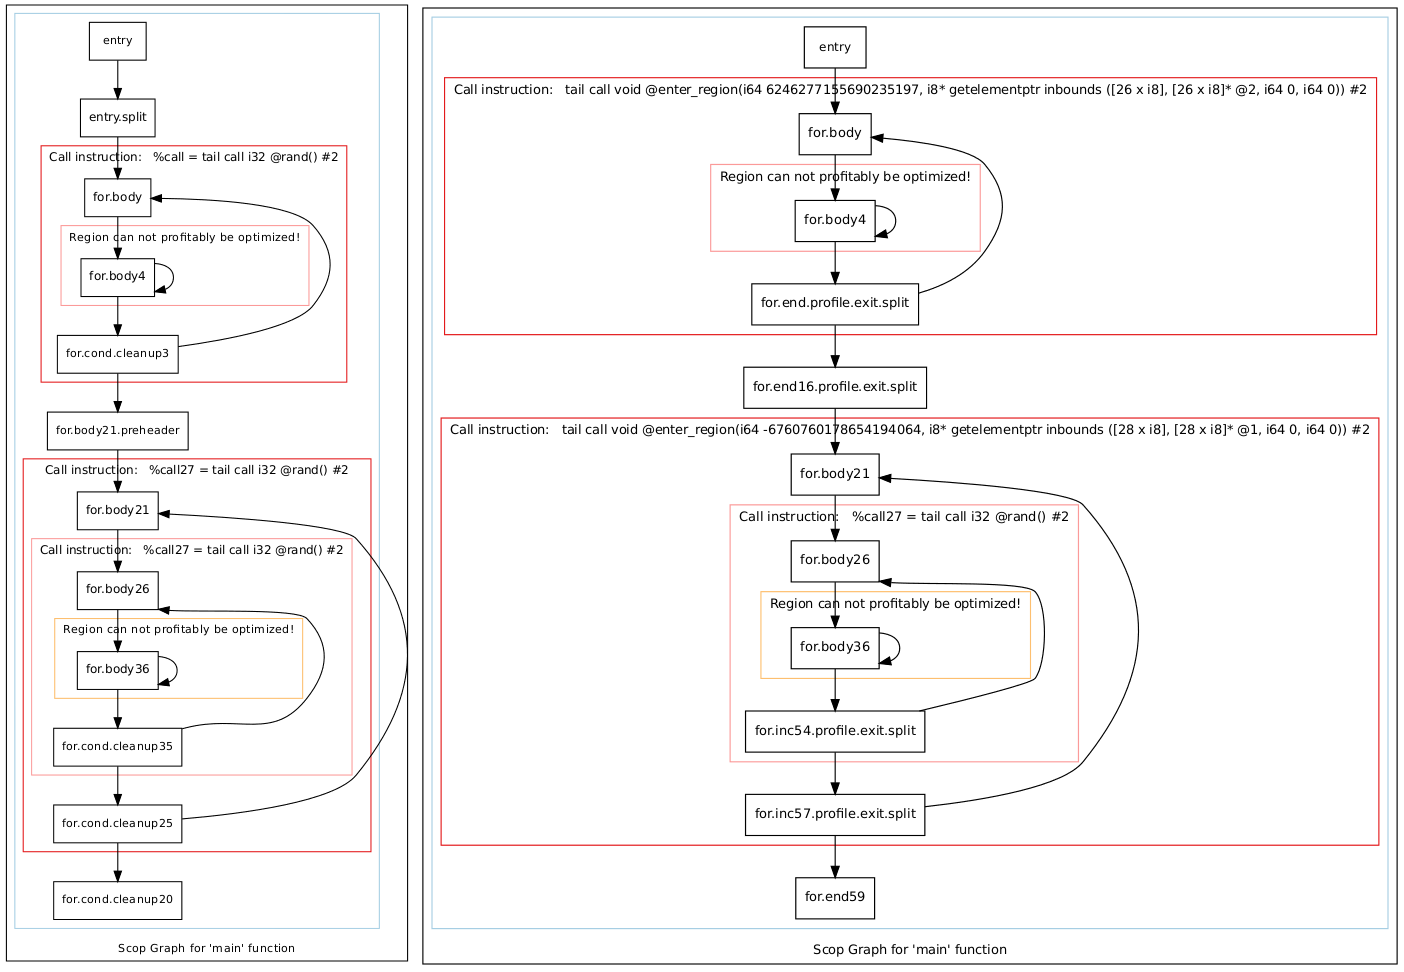
\includegraphics[height=\textheight]{gfx/matmulScopsAfterInstrumentation.png}
\end{frame}
\subsection{Überdeckung der SCoPs}
\begin{frame}{\subsecname: \(DynCov_s\) und \(DynCov_p\)}
    \vspace{-1cm}
    \begin{columns}
        \begin{column}{5cm}
            \begin{figure}[!h]
                \includesvg[height=\textheight]{compDyncovScopParent}
            \end{figure}
        \end{column}
        \begin{column}{5cm}
            \begin{itemize}[<+(1)->]
                \item Unteren 25\% bleiben gleich
                \item Sonst leichter Anstieg der Überdeckung
                \item ABER: \textbf{Nicht signifikant}
            \end{itemize}
        \end{column}
    \end{columns}
\end{frame}
\subsection{Gründe für Ablehnung größerer Regions}
\begin{frame}{\subsecname}
    \vspace{-0.2cm}
    \begin{figure}[!h]
        \includesvg[height=\textheight]{pieInvalidReasons}
    \end{figure}
\end{frame}
\begin{frame}{Analyse bzgl. \subsecname}
    \centering
    \pspicture(0, .18\textheight)
        \rput(.5\textwidth,.5\textheight){
            \includesvg[height=\textheight]{pieInvalidReasons}
        }
        \rput(0, 0){
            \transparent{.8}\textcolor{white}{\rule{\paperwidth}{.82\paperheight}}
        }
        \rput(0, 0){
            \begin{minipage}{\textwidth}
                \begin{description}[<+->]
                    \item[{\color[HTML]{b05900} toplevel regions}]Sind bereits \enquote{maximal}, wenn nicht in größerem Kontext betrachtet
                    \item[{\color[HTML]{ffba75} Could not compute}]Sind z.T. abhängig von Parametern, d.h. Auflösung schwierig
                    \item[{\color[HTML]{ff9933} Call instruction}]Vermutlich auch zukünftig keine Garantien von Seiteneffektfreiheit
                    \item[{\color[HTML]{0087b0} Non affine loop bound}]Oft nicht-Affinität zwingend\\
                        Ansätze für nicht-Affinität vorhanden, aber noch nicht vielversprechend
                    \item[{\color[HTML]{8ae3ff} Polly returned no reason}]Schwierig irgendwelche Aussagen zu treffen
                \end{description}\pause
                \(\Rightarrow\) \textbf{Bereits 87\% überdeckt}
            \end{minipage}
        }
    \endpspicture
\end{frame}
\subsection{Theoretischer Speedup}
\begin{frame}{\subsecname: Auswertung}
    Sei \(N=8\).
    \begin{itemize}[<+(1)->]
        \item Theoretischer Speedup SCoPs: 1.55
        \item Theoretischer Speedup MaxRegions: 1.61
    \end{itemize}\pause
    \(\Rightarrow\) \textbf{Nicht signifikant höher}
\end{frame}

\begin{frame}[plain]
    \begin{center}
        \Huge{Welche Fragen beschäftigen Sie noch?}\\
        \Large{Sie haben \textit{jetzt} Gelgenheit.}
    \end{center}
\end{frame}

\section{Quellen}
\begin{frame}[allowframebreaks]{\secname}
    \nocite{*}
    \printbibliography
\end{frame}

\end{document}
